\begin{frame}
\frametitle{Parallel Decomposition}
\framesubtitle{Recap}
\begin{itemize}
\item Data or Task parallelism encoded in objects
\item Object count independent of processors
\item How many objects, then? How big?
\end{itemize}
\end{frame}

\begin{frame}
\frametitle{Parallel Decomposition}
\framesubtitle{Overdecomposition}
Want \emph{several} objects per processor
\begin{itemize}
\item Increase chance that one will have work available
\item Overlap communication of one with computation of another
\item Important for later optimizations
\end{itemize}
\end{frame}

\begin{frame}[fragile]
\frametitle{Parallel Decomposition}
\framesubtitle{Overdecomposition Example: Weather Forecasting in BRAMS}
\begin{itemize}
 \item BRAMS: Brazillian weather code (based on RAMS)
 \item AMPI version (Eduardo Rodrigues, with C. Mendes and J. Panetta)
\end{itemize}
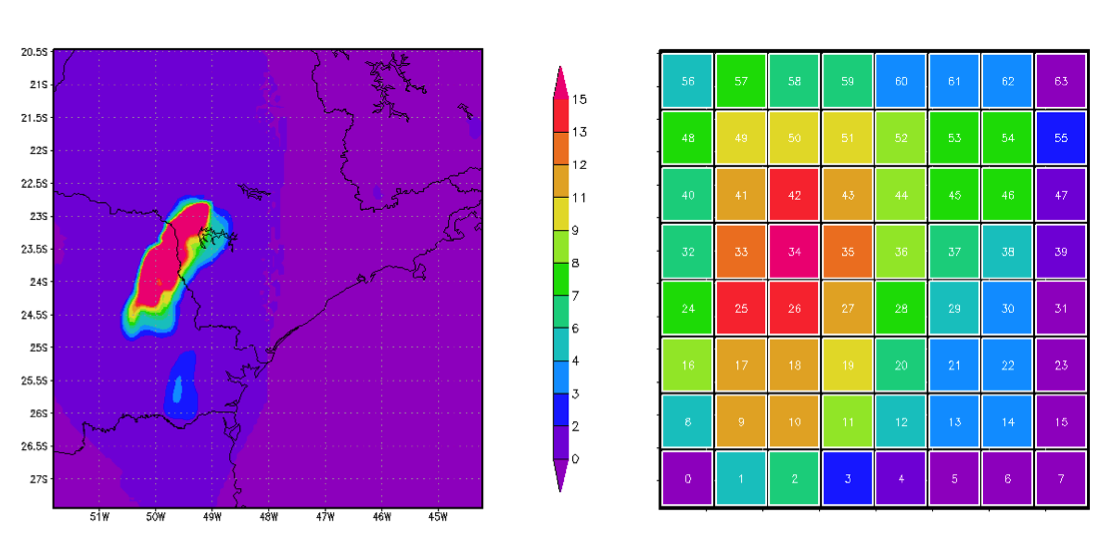
\includegraphics[width=0.9\textwidth]{../figures/bramsVisual.png}
\end{frame}


\begin{frame}[fragile]
\frametitle{Basic Virtualization of BRAMS}
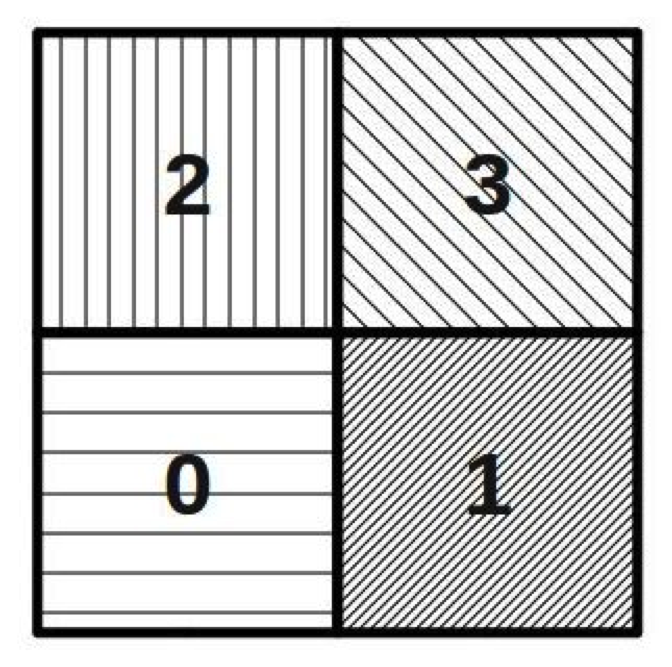
\includegraphics[width=0.5\textwidth]{../figures/bramsNonVirtual.png}
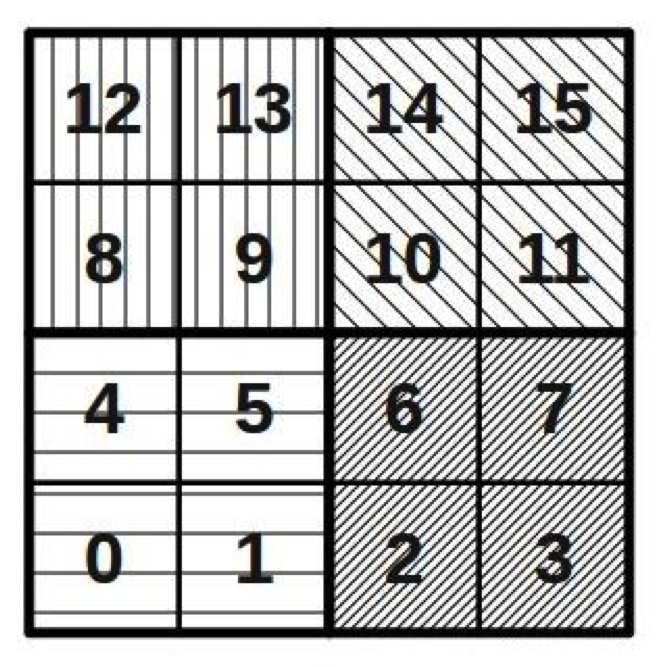
\includegraphics[width=0.5\textwidth]{../figures/bramsVirtual.png}
\end{frame}

\begin{frame}[fragile]
\frametitle{Baseline: 64 objects on 64 processors}
\begin{center}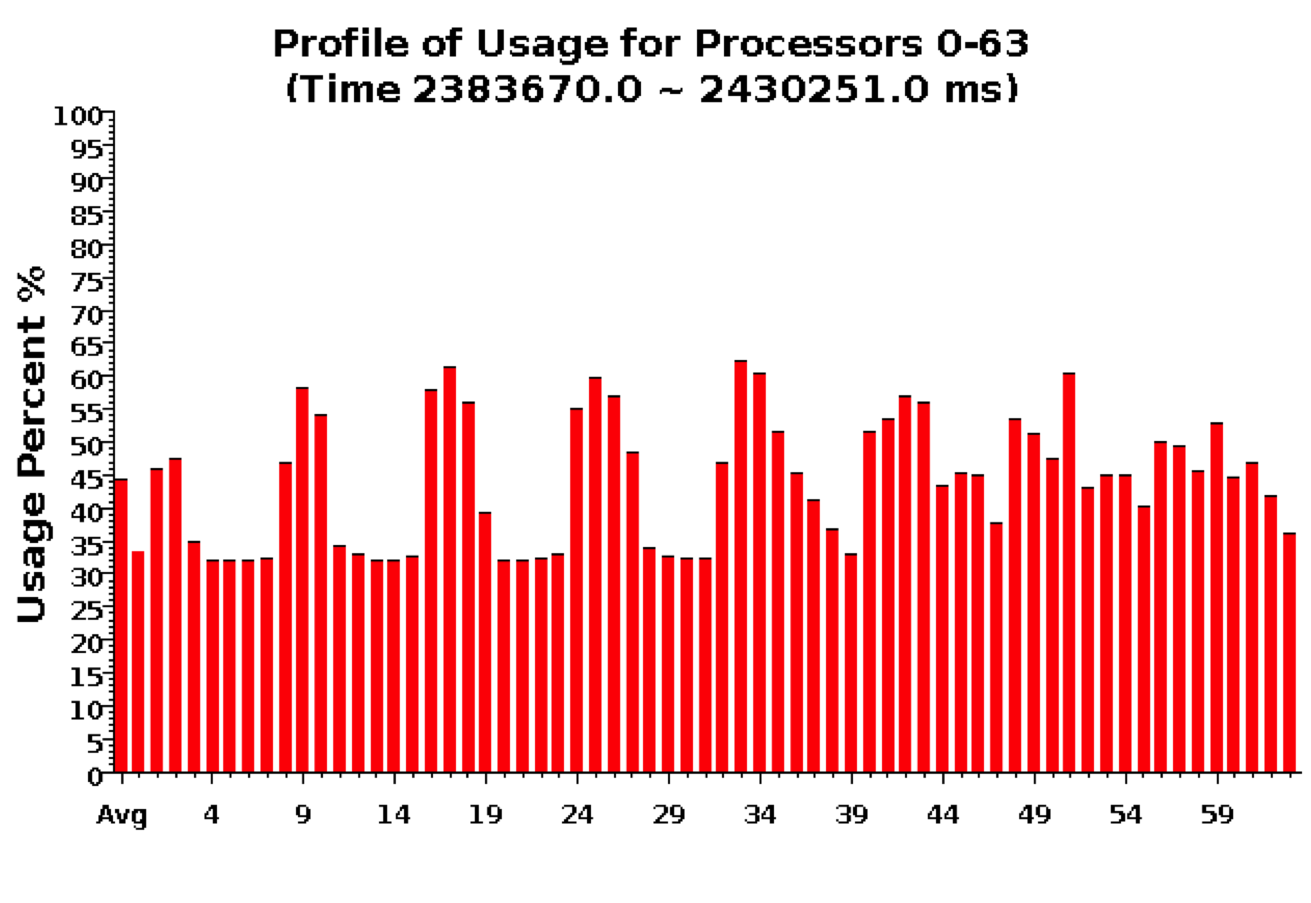
\includegraphics[width=0.9\textwidth]{../figures/usageNonVirtual.png}\end{center}
\end{frame}

\begin{frame}[fragile]
\frametitle{Over-decomposition: 1024 objects on 64 processors}
\framesubtitle{Benefits from communication/computation overlap}
\begin{center}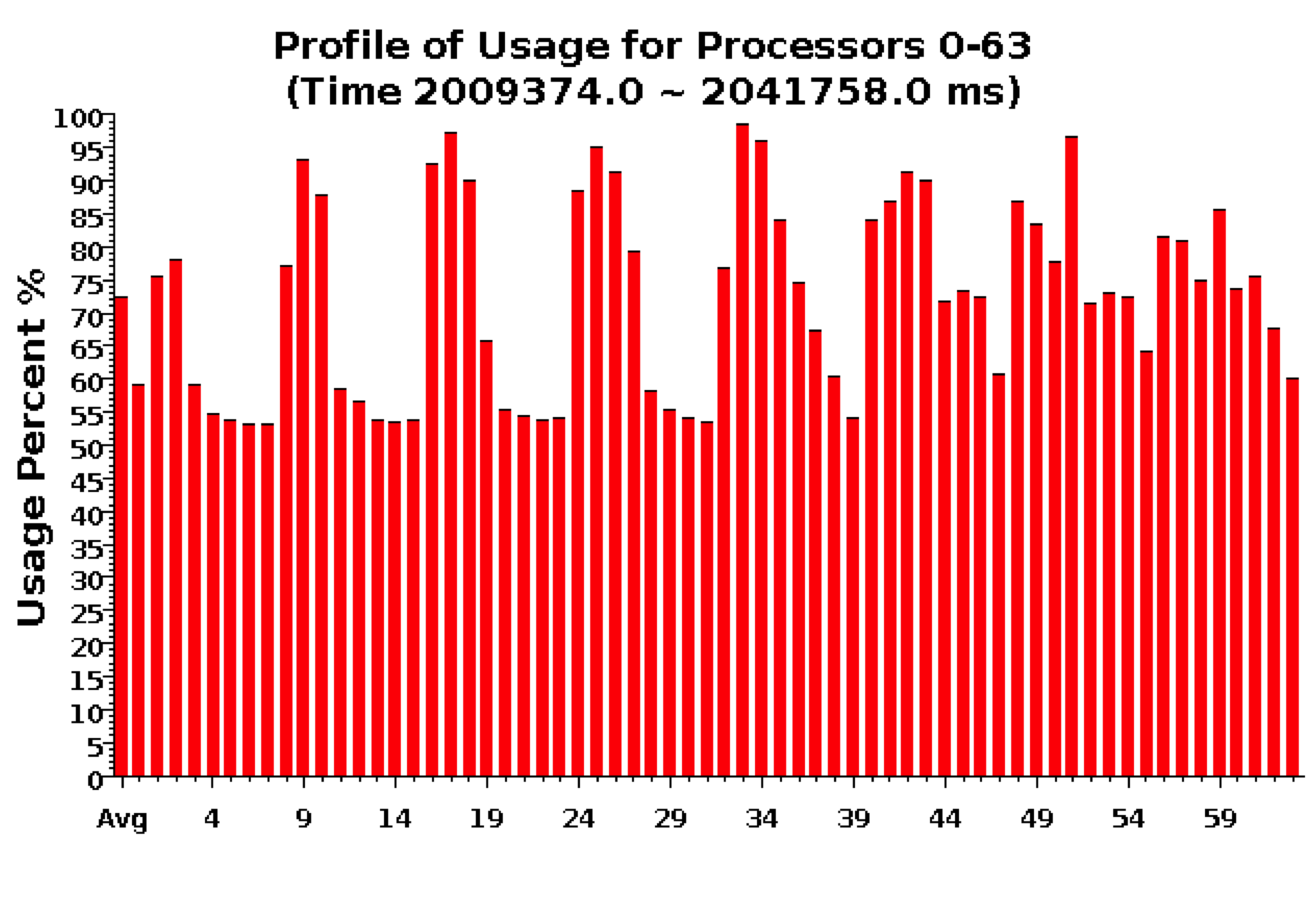
\includegraphics[width=0.9\textwidth]{../figures/usageVirtual.png}\end{center}
\end{frame}


\begin{frame}[fragile]
\frametitle{With Load Balancing: 1024 objects on 64 processors}
\begin{center}
\begin{itemize}
\item No overdecomp (64 threads): 4988 sec
\item Overdecomp into 1024 threads: 3713 sec
\item Load balancing (1024 threads): 3367 sec
\end{itemize}
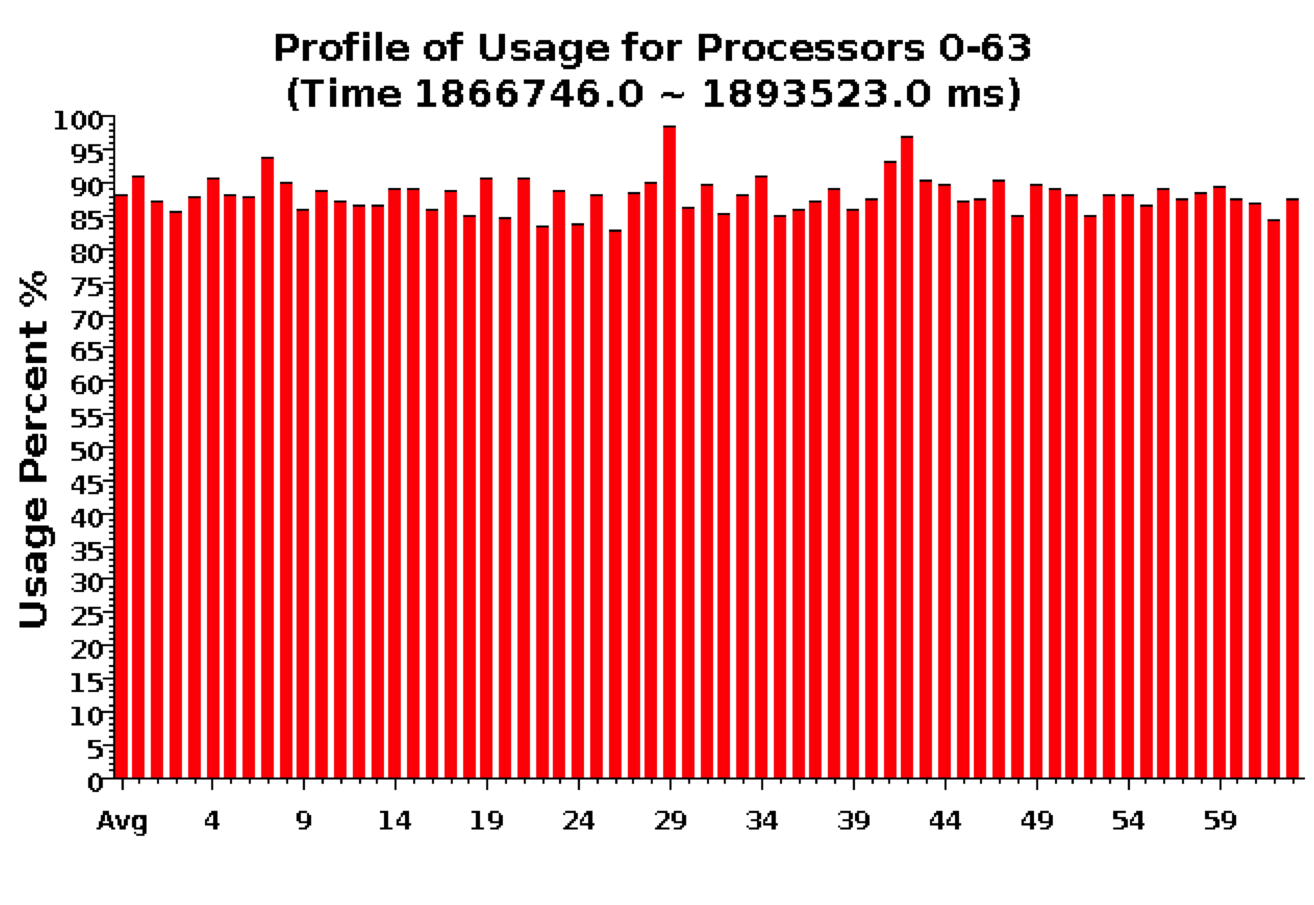
\includegraphics[width=0.8\textwidth]{../figures/usageLB.png}
\end{center}
\end{frame}

\begin{frame}
\frametitle{Grain Size}
  \begin{itemize}
    \item (working) Definition: the amount of computation per potentially
      parallel event (task creation, enqueue/dequeue, messaging,
      locking, etc.)
  \end{itemize}
  \begin{center} 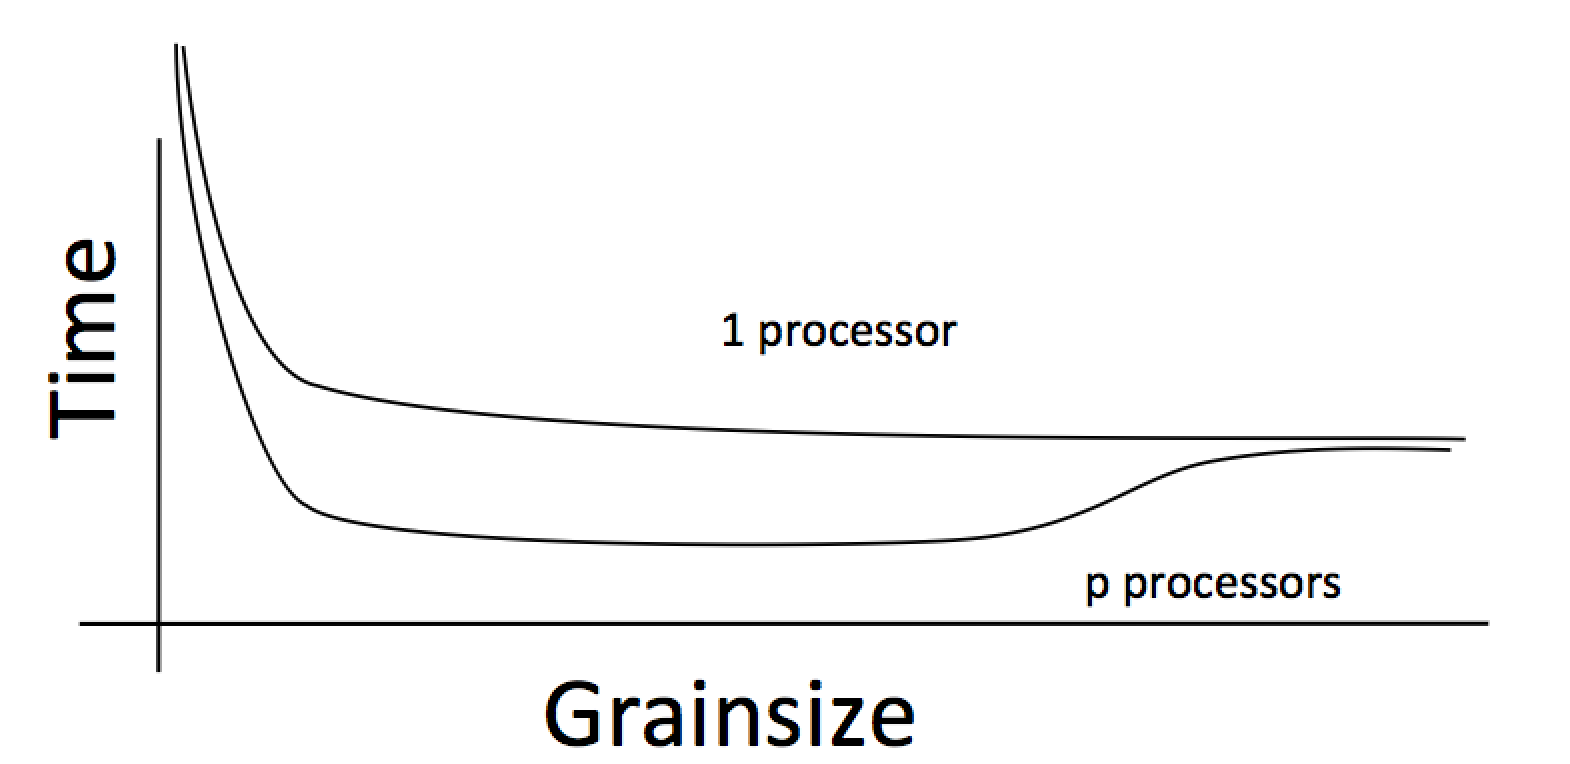
\includegraphics[width=0.7\textwidth]{../figures/grain1.png} \end{center}
\end{frame}
